\documentclass[12pt]{article}
\usepackage{silence}
\WarningFilter{xepersian}{Font}
\WarningFilter{fontspec}{font-not-found}

\usepackage{amsmath}
\usepackage{amssymb}
\usepackage{graphicx}
\usepackage{geometry}
\usepackage{listings}
\usepackage{xcolor}
\usepackage{caption}

\geometry{a4paper, margin=1in}

\lstset{
 language=Python,
 basicstyle=\ttfamily\small,
 keywordstyle=\color{blue},
 commentstyle=\color{green!50!black},
 stringstyle=\color{red},
 numbers=left,
 numberstyle=\tiny\color{gray},
 stepnumber=1,
 numbersep=8pt,
 backgroundcolor=\color{gray!5},
 showstringspaces=false,
 tabsize=4,
 frame=single,
 breaklines=true
}

\usepackage{xepersian}
\settextfont{B Nazanin}
\setlatintextfont{Times New Roman}

\begin{document}

\begin{titlepage}
\centering
\vspace*{2cm}
{\Large گزارش پروژه نرم‌افزار ریاضی\par}
\vspace{1cm}
{\large امیرمحمد ذاکر\par}
\vfill
{\large \today\par}
\end{titlepage}

\tableofcontents
\clearpage

 \section{درونیابی لاگرانژ و اسپلاین مکعبی}
 در این بخش، هدف یافتن توابع درونیاب برای نقاط داده‌شده در صورت پروژه است. نقاط مشخص‌شده عبارتند از:
 $ (1,1) $، $ (2,3) $، $ (3,5) $، $ (4,8) $، $ (5,5) $ و $ (6,2) $.
 برای این داده‌ها، دو روش درونیابی لاگرانژ\footnote{\lr{Lagrange Interpolation}} و اسپلاین مکعبی طبیعی\footnote{\lr{Natural Cubic Spline}} در محیط پایتون\footnote{\lr{Python}} پیاده‌سازی شده است.
 
 \subsection{مراحل و نحوه پیاده‌سازی الگوریتم‌ها}
 پروژه پایتون مربوط به این بخش شامل گام‌های زیر است:
 \begin{enumerate}
  \item \textbf{تعریف و مقداردهی اولیه نقاط:} ابتدا نقاط به‌صورت دو آرایه مجزا برای مولفه‌های $ x $ و $ y $ در کتابخانه نام‌پای\footnote{\lr{NumPy}} تعریف می‌شوند.
  \item \textbf{درونیابی لاگرانژ:} برای درونیابی لاگرانژ و جلوگیری از ناپایداری‌های عددی معمول، از کلاس پیشرفته \lstinline|BarycentricInterpolator| در کتابخانه سای‌پای\footnote{\lr{SciPy}} استفاده شده است.
  \item \textbf{استخراج محاسباتی ضابطه ریاضی:} به دلیل اینکه کتابخانه‌های محاسبات عددی صرفاً خروجی عددی می‌دهند، با استفاده از کتابخانه سیم‌پای\footnote{\lr{SymPy}} فرمول نمادین پایه‌های لاگرانژ پیاده‌سازی و در نهایت با دستور \lstinline|expand| ساده‌سازی شده است تا ضابطه دقیق باز شود.
  \item \textbf{درونیابی اسپلاین مکعبی:} با استفاده از کلاس \lstinline|CubicSpline| و با تنظیم پارامتر \lstinline|bc_type='natural'| شرط مرزی صفر بودن مشتق دوم در نقاط ابتدایی و انتهایی اعمال شده و ضرایب توابع تکه‌ای استخراج گردیده‌اند.
  \item \textbf{تصویرسازی و ذخیره‌سازی:} با کمک کتابخانه مت‌پلات‌لیب\footnote{\lr{Matplotlib}} هر دو نمودار به همراه نقاط اصلی رسم و با کیفیت بالا ذخیره می‌شوند.
 \end{enumerate}
 
 \subsection{کد پایتون پیاده‌سازی شده}
 کد کامل پایتون که برای انجام محاسبات این بخش نوشته شده، به شرح زیر است:
 
 \begin{latin}
  \begin{lstlisting}
   import numpy as np
   import matplotlib.pyplot as plt
   from scipy.interpolate import BarycentricInterpolator, CubicSpline
   from sympy import symbols, expand
   
   # 1. Define the data points given in the project prompt
   x_data = np.array([1, 2, 3, 4, 5, 6])
   y_data = np.array([1, 3, 5, 8, 5, 2])
   
   print("--- Part 1: Lagrange Interpolation ---")
   # 2. Perform Lagrange interpolation using BarycentricInterpolator
   lagrange_interpolator = BarycentricInterpolator(x_data, y_data)
   
   # Extract the exact mathematical formula using sympy for clear display
   x_sym = symbols('x')
   lagrange_expr = 0
   for i in range(len(x_data)):
       # Construct Lagrange basis polynomials
       p = 1
       for j in range(len(x_data)):
           if i != j:
               p *= (x_sym - x_data[j]) / (x_data[i] - x_data[j])
       lagrange_expr += y_data[i] * p
   
   lagrange_simplified = expand(lagrange_expr)
   print("Exact formula for Lagrange interpolating polynomial:")
   print(f"L(x) = {lagrange_simplified}\n")
   
   print("--- Part 2: Spline Interpolation ---")
   # 3. Perform Cubic Spline interpolation (Natural type)
   cs = CubicSpline(x_data, y_data, bc_type='natural')
   
   print("Exact piecewise formulas for the Cubic Spline (per interval):")
   for i in range(len(x_data) - 1):
       coeffs = cs.c[:, i]
       d, c, b, a = coeffs[0], coeffs[1], coeffs[2], coeffs[3]
       print(f"Interval [{x_data[i]}, {x_data[i+1]}]:")
       print(f"  S_{i}(x) = {a} + {b:.4f}(x - {x_data[i]}) + {c:.4f}(x - {x_data[i]})^2 + {d:.4f}(x - {x_data[i]})^3")
			
   # 4. Plotting the results for the final report
   x_plot = np.linspace(1, 6, 500)
   y_lagrange_plot = lagrange_interpolator(x_plot)
   y_spline_plot = cs(x_plot)
			
   plt.figure(figsize=(10, 6))
   plt.scatter(x_data, y_data, color='red', zorder=5, label='Original Data Points')
   plt.plot(x_plot, y_lagrange_plot, label='Lagrange Interpolation', linestyle='--', color='blue')
   plt.plot(x_plot, y_spline_plot, label='Natural Cubic Spline', linestyle='-', color='green')
   plt.title('Comparison of Lagrange and Cubic Spline Interpolation')
   plt.xlabel('X')
   plt.ylabel('Y')
   plt.grid(True, linestyle=':', alpha=0.6)
   plt.legend()
   plt.savefig('interpolation_plot.png', dpi=300)
  \end{lstlisting}
 \end{latin}
	
 \subsection{خروجی دقیق برنامه در محیط ترمینال}
 پس از اجرای کد فوق، خروجی‌های دقیق ریاضی به صورت متنی در ترمینال به شرح زیر نمایش داده می‌شوند:
	
 \begin{latin}
  \begin{verbatim}
   --- Part 1: Lagrange Interpolation ---
   Exact formula for Lagrange interpolating polynomial:
   L(x) = 7*x**5/40 - 71*x**4/24 + 147*x**3/8 - 1249*x**2/24 + 1369*x/20 - 31
			
   --- Part 2: Spline Interpolation ---
   Exact piecewise formulas for the Cubic Spline (per interval):
   Interval [1, 2]:
     S_0(x) = 1.0 + 2.1866(x - 1) + 0.0000(x - 1)^2 + -0.1866(x - 1)^3
   Interval [2, 3]:
     S_1(x) = 3.0 + 1.6268(x - 2) + -0.5598(x - 2)^2 + 0.9330(x - 2)^3
   Interval [3, 4]:
     S_2(x) = 5.0 + 3.3062(x - 3) + 2.2392(x - 3)^2 + -2.5455(x - 3)^3
   Interval [4, 5]:
     S_3(x) = 8.0 + 0.1483(x - 4) + -5.3971(x - 4)^2 + 2.2488(x - 4)^3
   Interval [5, 6]:
     S_4(x) = 5.0 + -3.8995(x - 5) + 1.3493(x - 5)^2 + -0.4498(x - 5)^3
  \end{verbatim}
 \end{latin}
	
 \subsection{ضابطه چندجمله‌ای درونیاب لاگرانژ}
 با توجه به خروجی سیستم، ضابطه دقیق ریاضی ساده‌شده‌ی چندجمله‌ای لاگرانژ به صورت زیر است:
 \[
 L(x) = \frac{7}{40}x^5 - \frac{71}{24}x^4 + \frac{147}{8}x^3 - \frac{1249}{24}x^2 + \frac{1369}{20}x - 31.
 \]
	
 \subsection{ضابطه تکه‌ای درونیاب اسپلاین مکعبی}
 فرمول ریاضی تکه‌ای توابع درجه سوم برازش‌شده بر روی فواصل مجاور به شرح زیر است:
 \begin{align*}
  S_0(x) &= 1.0 + 2.1866(x - 1) - 0.1866(x - 1)^3, \quad & x \in [1, 2], \\
  S_1(x) &= 3.0 + 1.6268(x - 2) - 0.5598(x - 2)^2 + 0.9330(x - 2)^3, \quad & x \in [2, 3], \\
  S_2(x) &= 5.0 + 3.3062(x - 3) + 2.2392(x - 3)^2 - 2.5455(x - 3)^3, \quad & x \in [3, 4], \\
  S_3(x) &= 8.0 + 0.1483(x - 4) - 5.3971(x - 4)^2 + 2.2488(x - 4)^3, \quad & x \in [4, 5], \\
  S_4(x) &= 5.0 - 3.8995(x - 5) + 1.3493(x - 5)^2 - 0.4498(x - 5)^3, \quad & x \in [5, 6].
 \end{align*}
	
 \subsection{نمودار مقایسه‌ای و تحلیل کامل رفتار توابع}
 شکل~\ref{fig:interpolation} نشان‌دهنده نمودار خروجی حاصل از اجرای کد پایتون است.
	
 \begin{figure}[htbp]
  \centering
  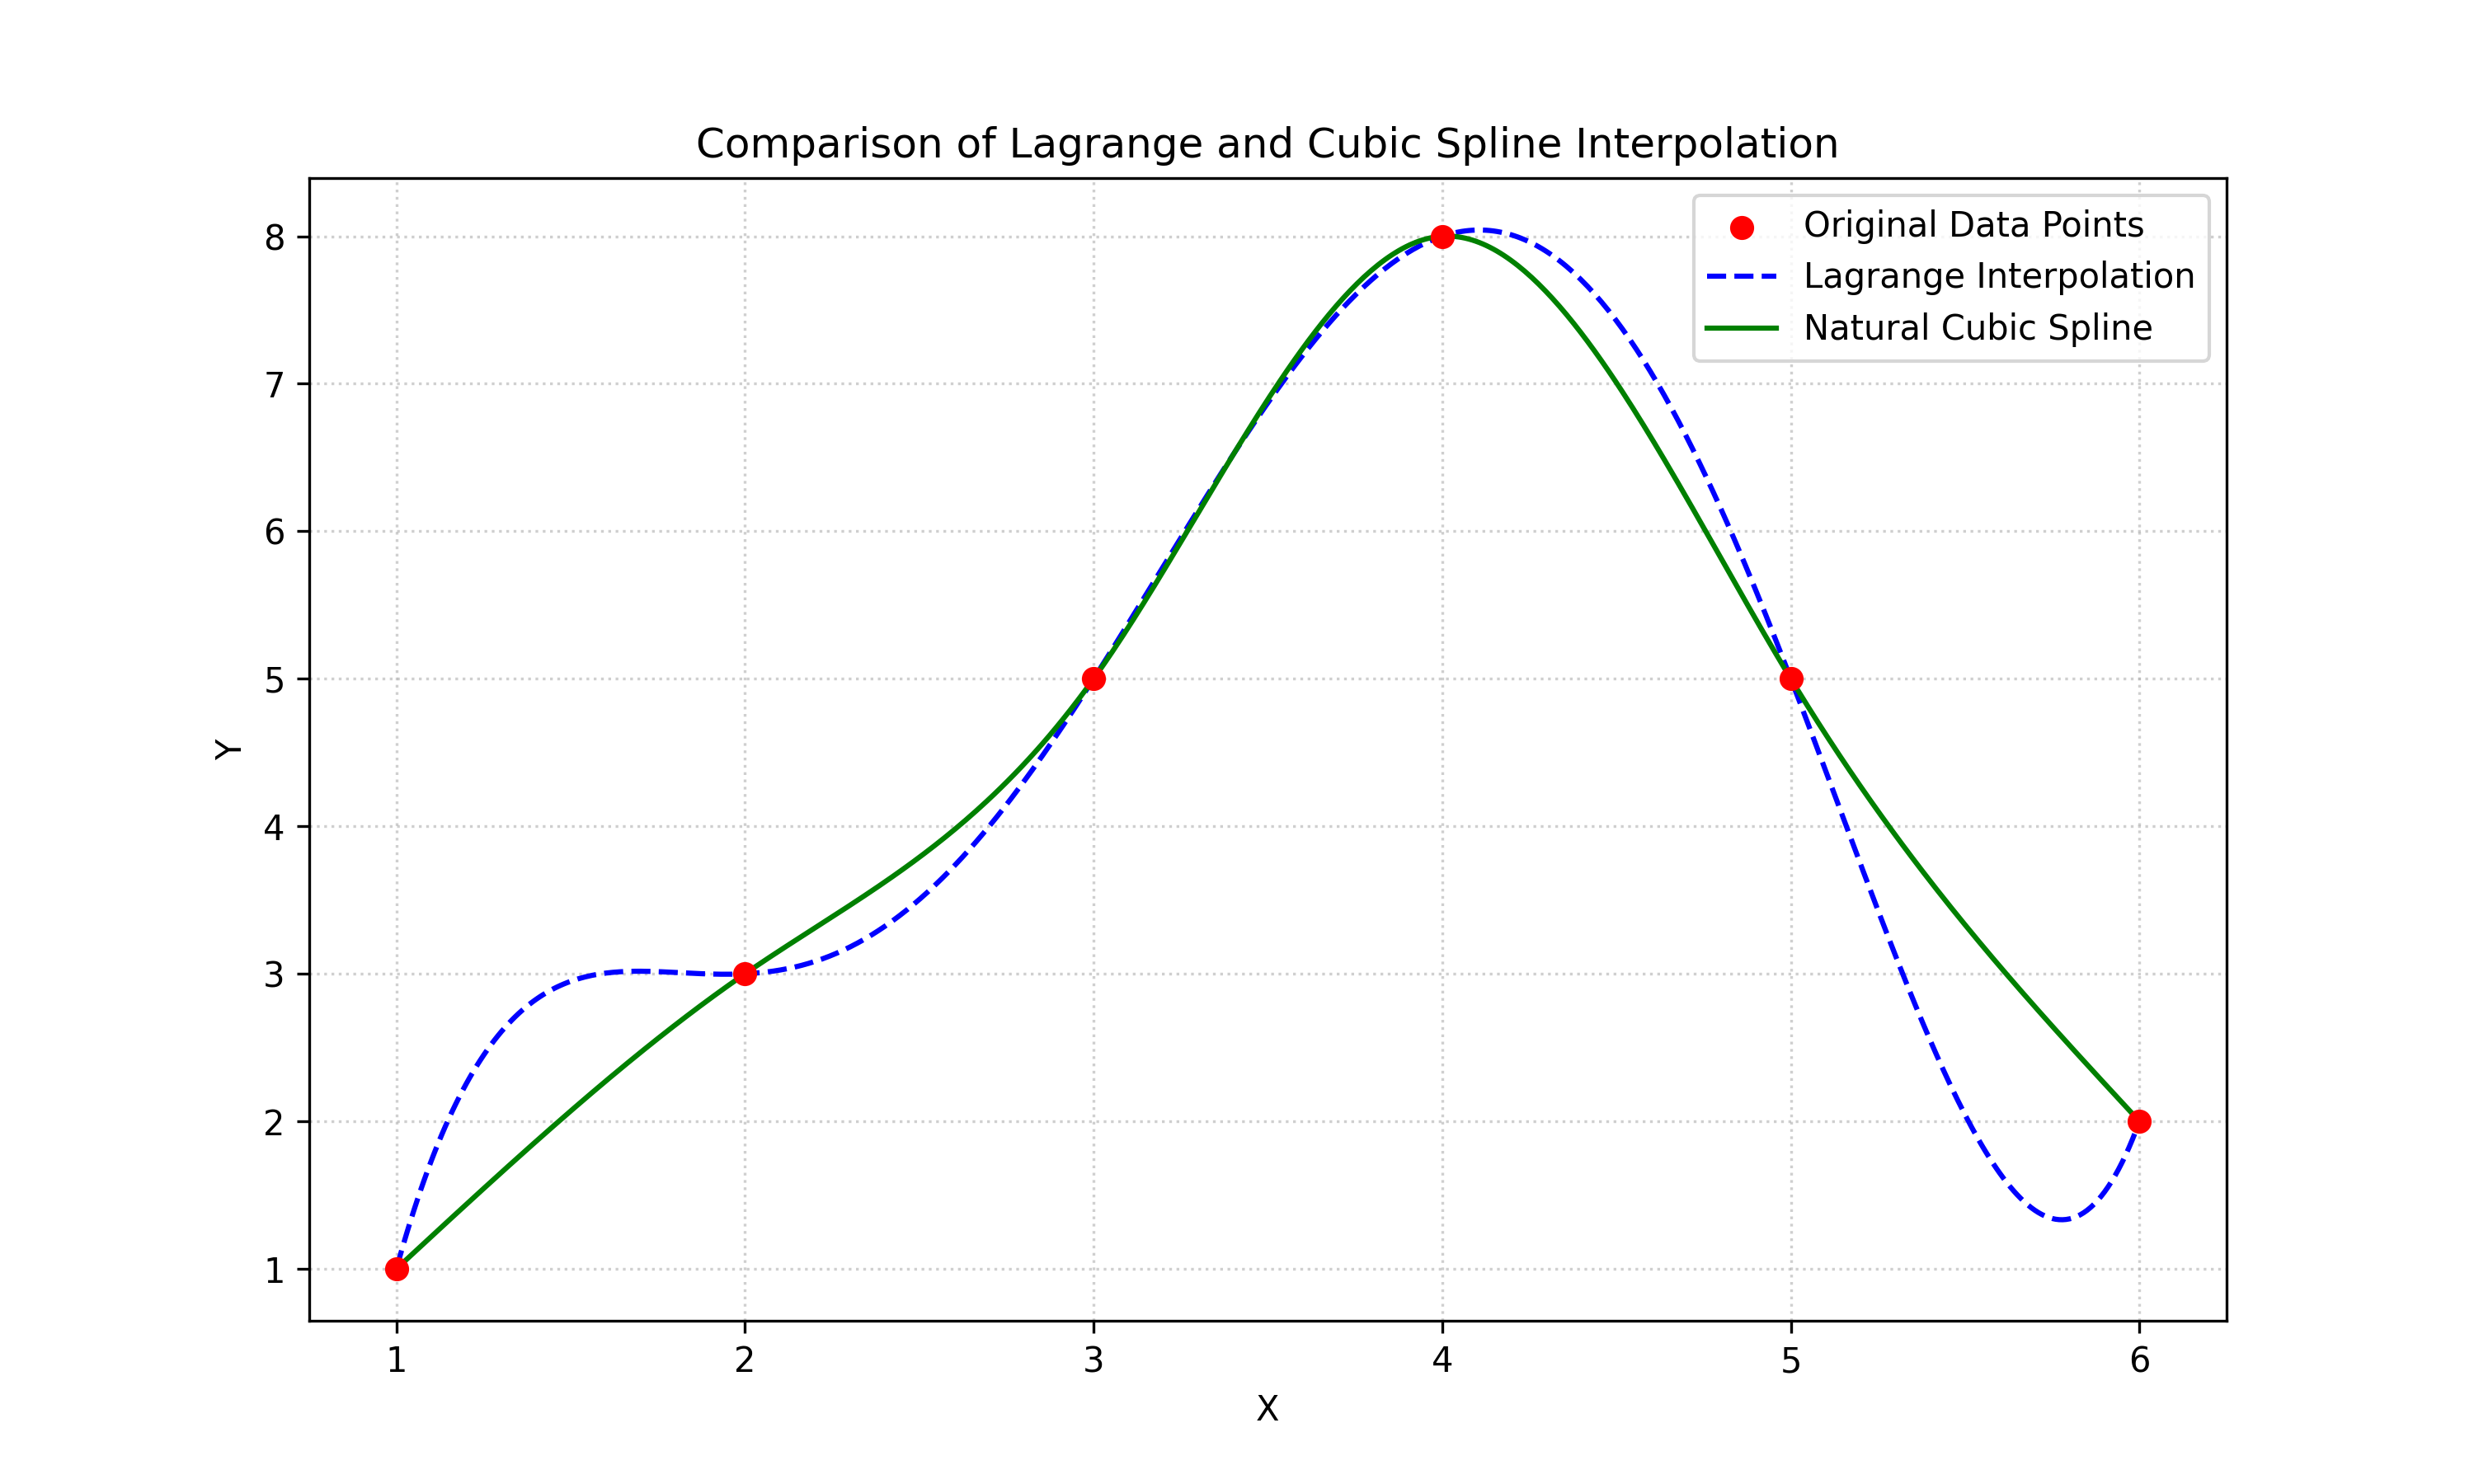
\includegraphics[width=0.85\textwidth]{interpolation_plot.png}
  \caption{نمودار مقایسه عملکرد درونیابی لاگرانژ و اسپلاین مکعبی طبیعی بر روی نقاط داده‌شده.}
  \label{fig:interpolation}
 \end{figure}
	
 تحلیل ریاضی رفتار این دو منحنی نشان می‌دهد که هر دو روش با موفقیت کامل از تمامی ۶ نقطه داده‌شده عبور کرده‌اند؛ اما تفاوت رفتار نوسانی عظیمی با یکدیگر دارند. چندجمله‌ای لاگرانژ به دلیل برخورداری از درجه بالا ($ n - 1 = 5 $)، در بازه‌های ابتدایی و انتهایی دچار نوسانات شدید خارج از محدوده داده‌ها شده است. این رفتار نوسانی نامطلوب به پدیده رانگ\footnote{\lr{Runge's phenomenon}} معروف است که نشان می‌دهد توابع چندجمله‌ای درجه بالا برای نقاط با فواصل مساوی گزینه‌ی مناسبی نیستند.
	
 در مقابل، روش اسپلاین مکعبی به دلیل ماهیت تکه‌ای بودن، در هر بازه تنها از توابع درجه ۳ استفاده می‌کند. برقراری شروط پیوستگی هم‌زمانِ تابع، مشتق اول و مشتق دوم در نقاط گره‌ای در کنار شرط مرزی طبیعی (صفر بودن مشتق دوم در پایانه‌ها)، سبب شده است تا منحنی اسپلاین رفتاری بسیار پایدار، نرم، عاری از هرگونه نوسان کاذب و کاملاً منطبق بر روند توزیع داده‌ها ارائه دهد.

\clearpage
\section{تحلیل آماری و تصویرسازی داده‌های زمان اجرای الگوریتم‌ها}
در این بخش، هدف بررسی هوشمند و پویای داده‌های مربوط به زمان اجرای سه الگوریتم مختلف بر حسب اندازه داده‌های ورودی از محدوده $ 100 $ الی $ 600 $ کیلوبایت و تحلیل تغییرات رفتار آن‌ها پس از افزودن سطر جدید $ 700 $ کیلوبایت است. تمامی این مراحل بدون هاردکد کردن داده‌ها و از طریق توابع پانداس\footnote{\lr{Pandas}} انجام شده است.

\subsection{مراحل و نحوه پیاده‌سازی الگوریتم‌ها}
مراحل پیاده‌سازی این بخش در زبان پایتون\footnote{\lr{Python}} به شرح زیر است:
\begin{enumerate}
    \item \textbf{فراخوانی پویا:} با استفاده از تابع \lstinline|pd.read_excel|، فایل داده‌ها مستقیماً خوانده شده و با متد \lstinline|str.strip| نام ستون‌ها پاک‌سازی می‌شوند تا فواصل خالی احتمالی باعث ایجاد خطا در محاسبات نگردند.
    \item \textbf{محاسبه شاخص‌های آماری:} پیش از اعمال تغییرات در ساختار فایل، میانگین ستون مربوط به الگوریتم ۲ محاسبه و ثبت می‌شود.
    \item \textbf{تزریق پویای داده‌ی جدید:} ردیف جدید مربوط به داده‌ی $ 700 $ کیلوبایت به کمک تابع \lstinline|pd.concat| به انتهای ماتریس داده‌ها افزوده می‌شود تا در اجرای مجدد، نمودارها به صورت خودکار به‌روزرسانی شوند.
    \item \textbf{تولید نمودارها:} با بهره‌گیری از کتابخانه‌های مت‌پلات‌لیب\footnote{\lr{Matplotlib}} و سی‌بورن\footnote{\lr{Seaborn}}، سه نمودار خطی، میله‌ای و جعبه‌ای برای تحلیل همه‌جانبه توزیع و روند داده‌ها رسم می‌شوند.
\end{enumerate}

\subsection{کد پایتون پیاده‌سازی شده}
کد کامل پایتون توسعه‌یافته برای این بخش به صورت زیر است:

\begin{latin}
\begin{lstlisting}
import pandas as pd
import matplotlib.pyplot as plt
import seaborn as sns

# Set style for professional-looking plots
sns.set_theme(style="whitegrid")

# 1. Reading the Excel file dynamically
excel_file = 'پروژه 3.xlsx'
df = pd.read_excel(excel_file)
df.columns = df.columns.str.strip()

# 2. Calculating the mean for Alg.2 (Before adding the new data row)
mean_alg2 = df['Alg.2'].mean()
print("--- Part 2 (c): Statistical Analysis ---")
print(f"Mean execution time for Alg.2 (100KB to 600KB): {mean_alg2:.2f}\n")

# 3. Dynamically appending new data row (700KB row)
new_row = {
    'Run time for different data size': '700KB',
    'Alg.1': 80,
    'Alg.2': 320,
    'Alg.3': 700
}
df = pd.concat([df, pd.DataFrame([new_row])], ignore_index=True)
print("--- Part 2 (b): Updated Dataframe with 700KB Row ---")
print(df)
print("\n")

size_col = df.columns[0]
algorithms = [col for col in df.columns if col != size_col]

# 4. Plotting Bar, Line, and Box Plots
# Line Plot
plt.figure(figsize=(10, 6))
for alg in algorithms:
    plt.plot(df[size_col], df[alg], marker='o', linewidth=2, label=alg)
plt.title('Execution Time Trend across Different Data Sizes', fontsize=14, fontweight='bold')
plt.xlabel('Data Size', fontsize=12)
plt.ylabel('Execution Time (ms)', fontsize=12)
plt.legend()
plt.tight_layout()
plt.savefig('execution_time_line_plot.png', dpi=300)

# Bar Plot
df_long = pd.melt(df, id_vars=[size_col], value_vars=algorithms, var_name='Algorithm', value_name='Execution Time')
plt.figure(figsize=(10, 6))
sns.barplot(data=df_long, x=size_col, y='Execution Time', hue='Algorithm', palette='muted')
plt.title('Comparison of Algorithm Execution Times per Data Size', fontsize=14, fontweight='bold')
plt.xlabel('Data Size', fontsize=12)
plt.ylabel('Execution Time (ms)', fontsize=12)
plt.tight_layout()
plt.savefig('execution_time_bar_plot.png', dpi=300)

# Box Plot
plt.figure(figsize=(8, 6))
sns.boxplot(data=df[algorithms], palette='pastel')
plt.title('Distribution of Execution Times per Algorithm', fontsize=14, fontweight='bold')
plt.xlabel('Algorithm', fontsize=12)
plt.ylabel('Execution Time Range', fontsize=12)
plt.tight_layout()
plt.savefig('execution_time_box_plot.png', dpi=300)
\end{lstlisting}
\end{latin}

\subsection{خروجی دقیق برنامه در محیط ترمینال}
متن خروجی حاصل از محاسبات و چاپ ماتریس داده‌ها به شرح زیر است:

\begin{latin}
\begin{verbatim}
--- Part 2 (c): Statistical Analysis ---
Mean execution time for Alg.2 (100KB to 600KB): 250.00

--- Part 2 (b): Updated Dataframe with 700KB Row ---
  Run time for different data size  Alg.1  Alg.2  Alg.3
0                            100KB     50    200    100
1                            200KB     55    220    200
2                            300KB     60    240    300
3                            400KB     65    260    400
4                            500KB     70    280    500
5                            600KB     75    300    600
6                            700KB     80    320    700
\end{verbatim}
\end{latin}

\subsection{تحلیل آماری میانگین زمان اجرا}
مطابق با خواسته بند «ج» پروژه، میانگین زمان اجرای مربوط به الگوریتم ۲ برای اندازه‌های اولیه داده‌ها ($ 100 $ تا $ 600 $ کیلوبایت) بر اساس فرمول زیر محاسبه شده است:
\[
\mu = \frac{1}{N}\sum_{i=1}^{N} X_i = \frac{200 + 220 + 240 + 260 + 280 + 300}{6} = 250.00\,\text{ms}.
\]
این شاخص آماری نشان می‌دهد که رفتار کلی الگوریتم ۲ در بازه داده‌های ورودی استاندارد، حول مرکز ثقل $ 250 $ میلی‌ثانیه نوسان می‌کند.

\subsection{نمودارهای ترسیم شده و تحلیل جامع رفتار الگوریتم‌ها}
نمودارهای زیر خروجی‌های تصویری به‌دست‌آمده از کد پایتون هستند که پس از تزریق خودکار داده‌ی سطر $ 700 $ کیلوبایت ترسیم شده‌اند.

\begin{figure}[htbp]
    \centering
    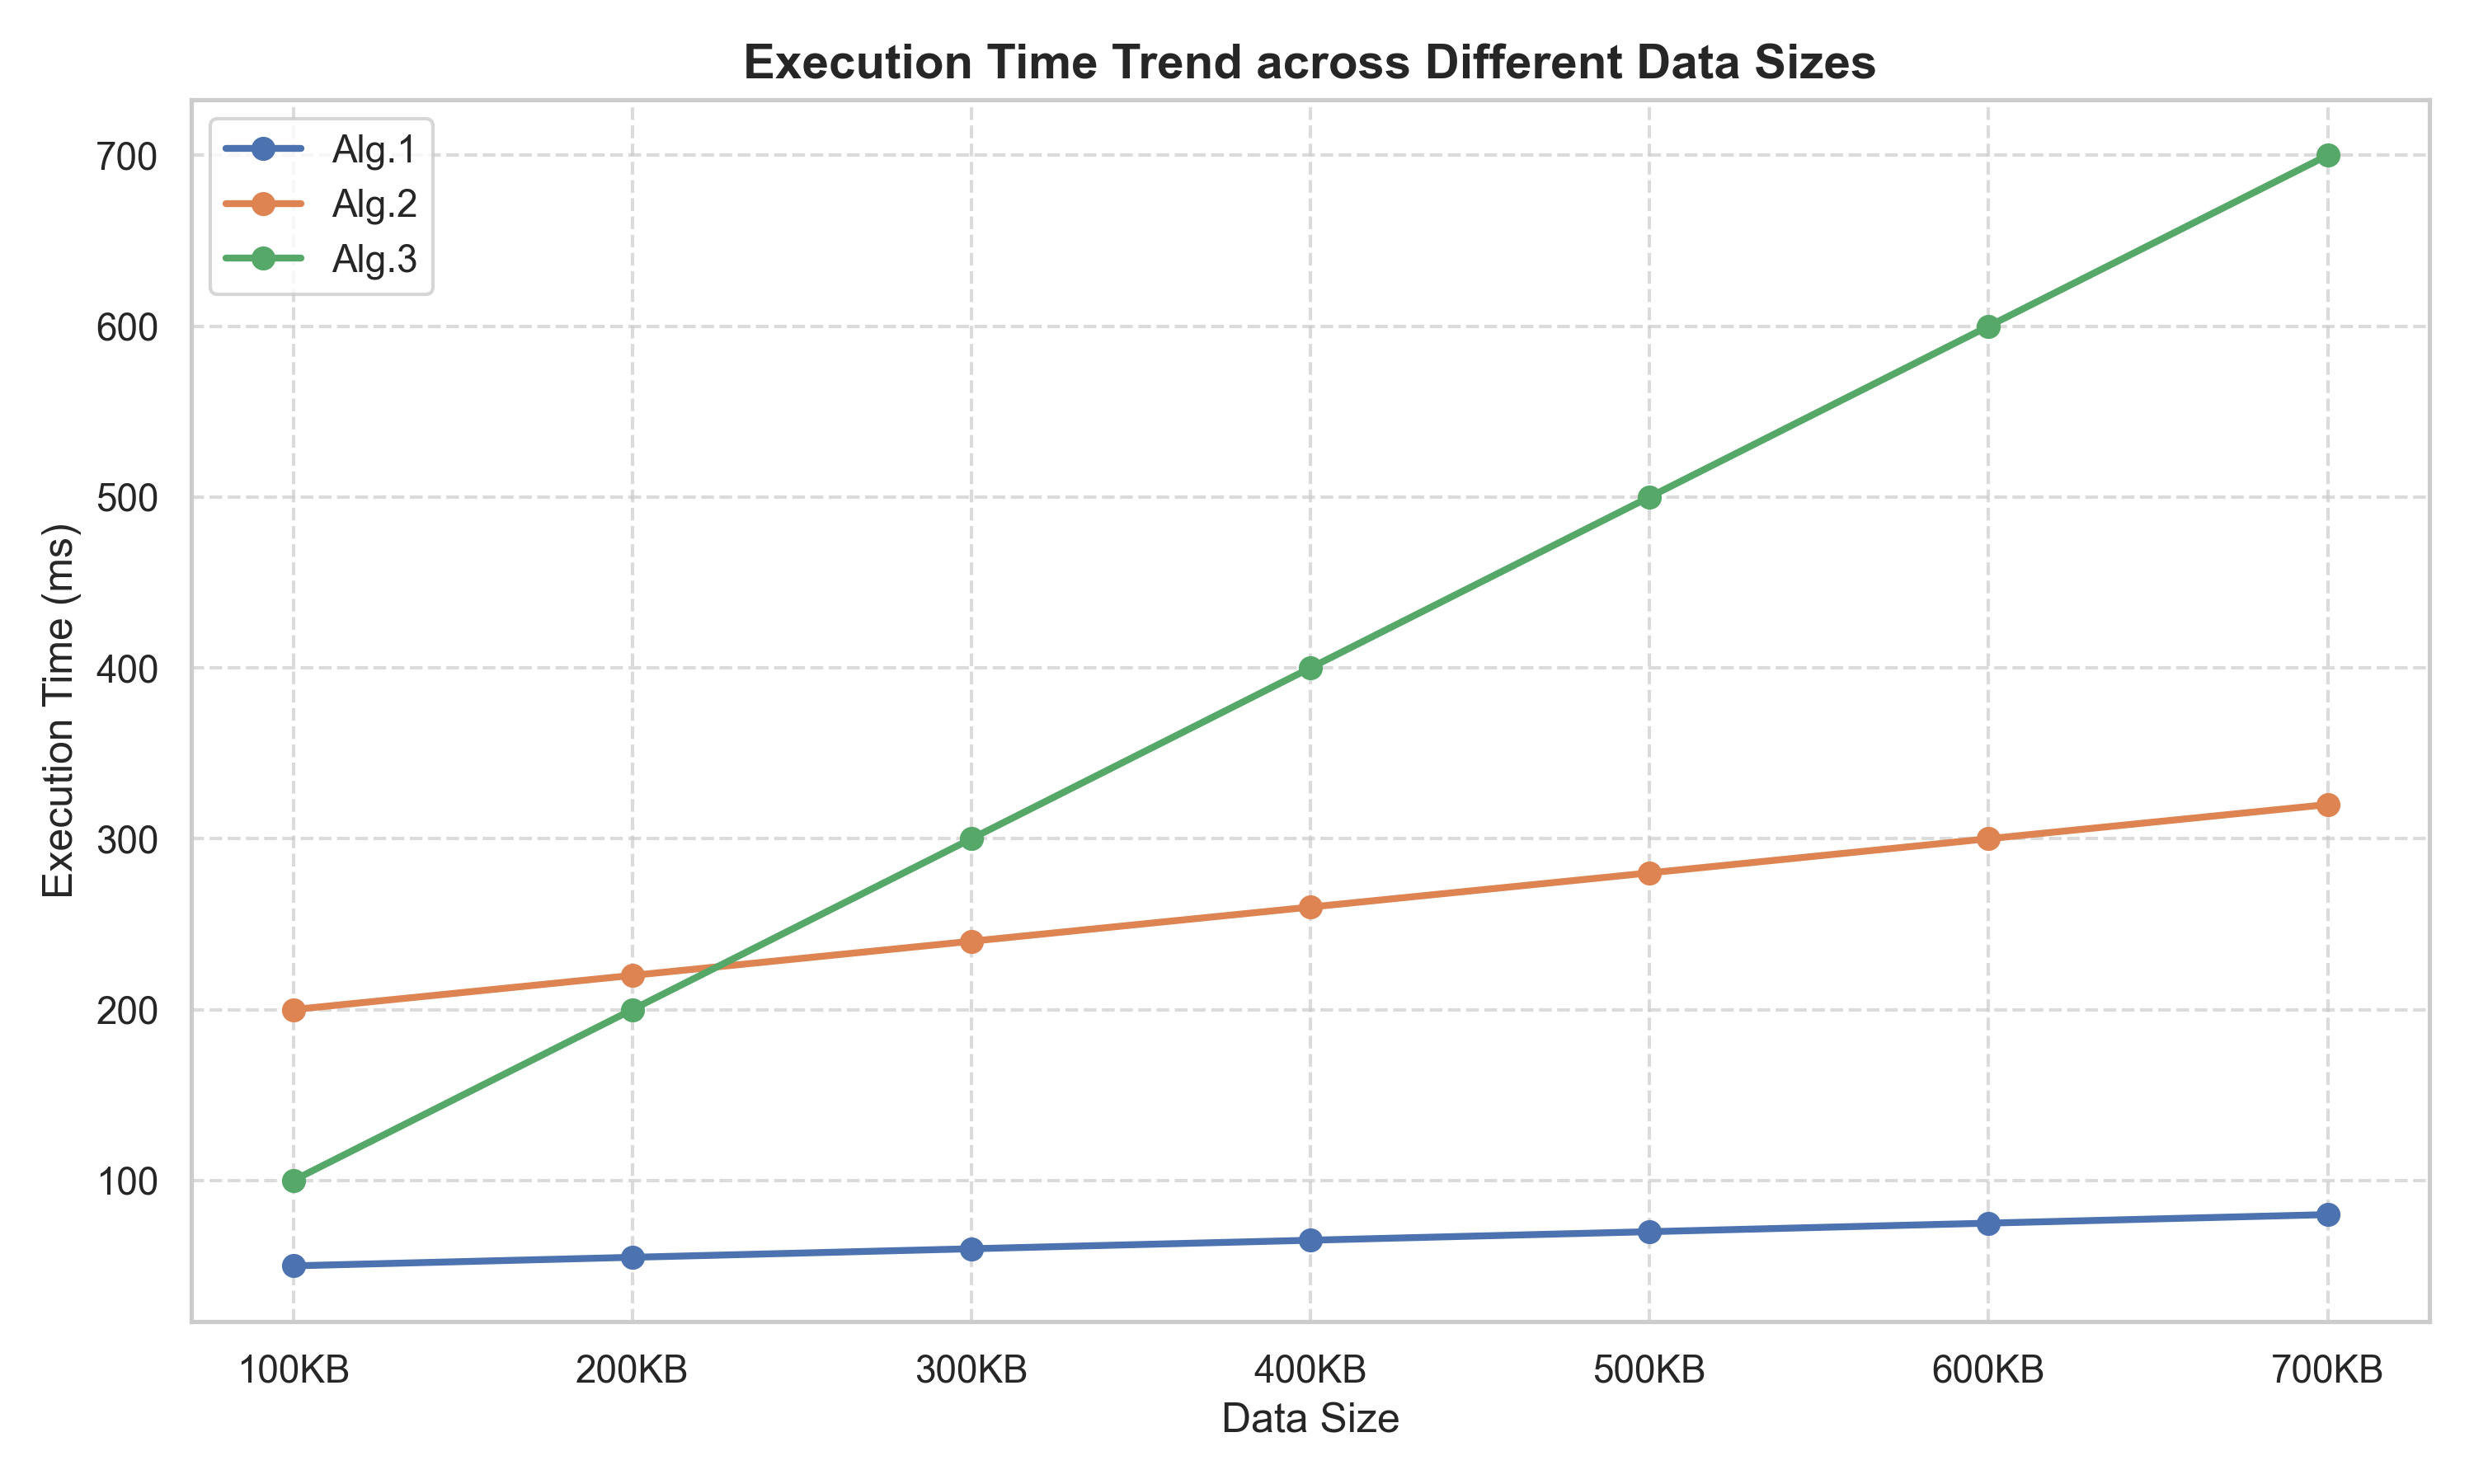
\includegraphics[width=0.85\textwidth]{execution_time_line_plot.png}
    \caption{روند تغییرات زمان اجرای الگوریتم‌ها بر حسب افزایش اندازه ورودی.}
    \label{fig:line_plot}
\end{figure}

\begin{figure}[htbp]
    \centering
    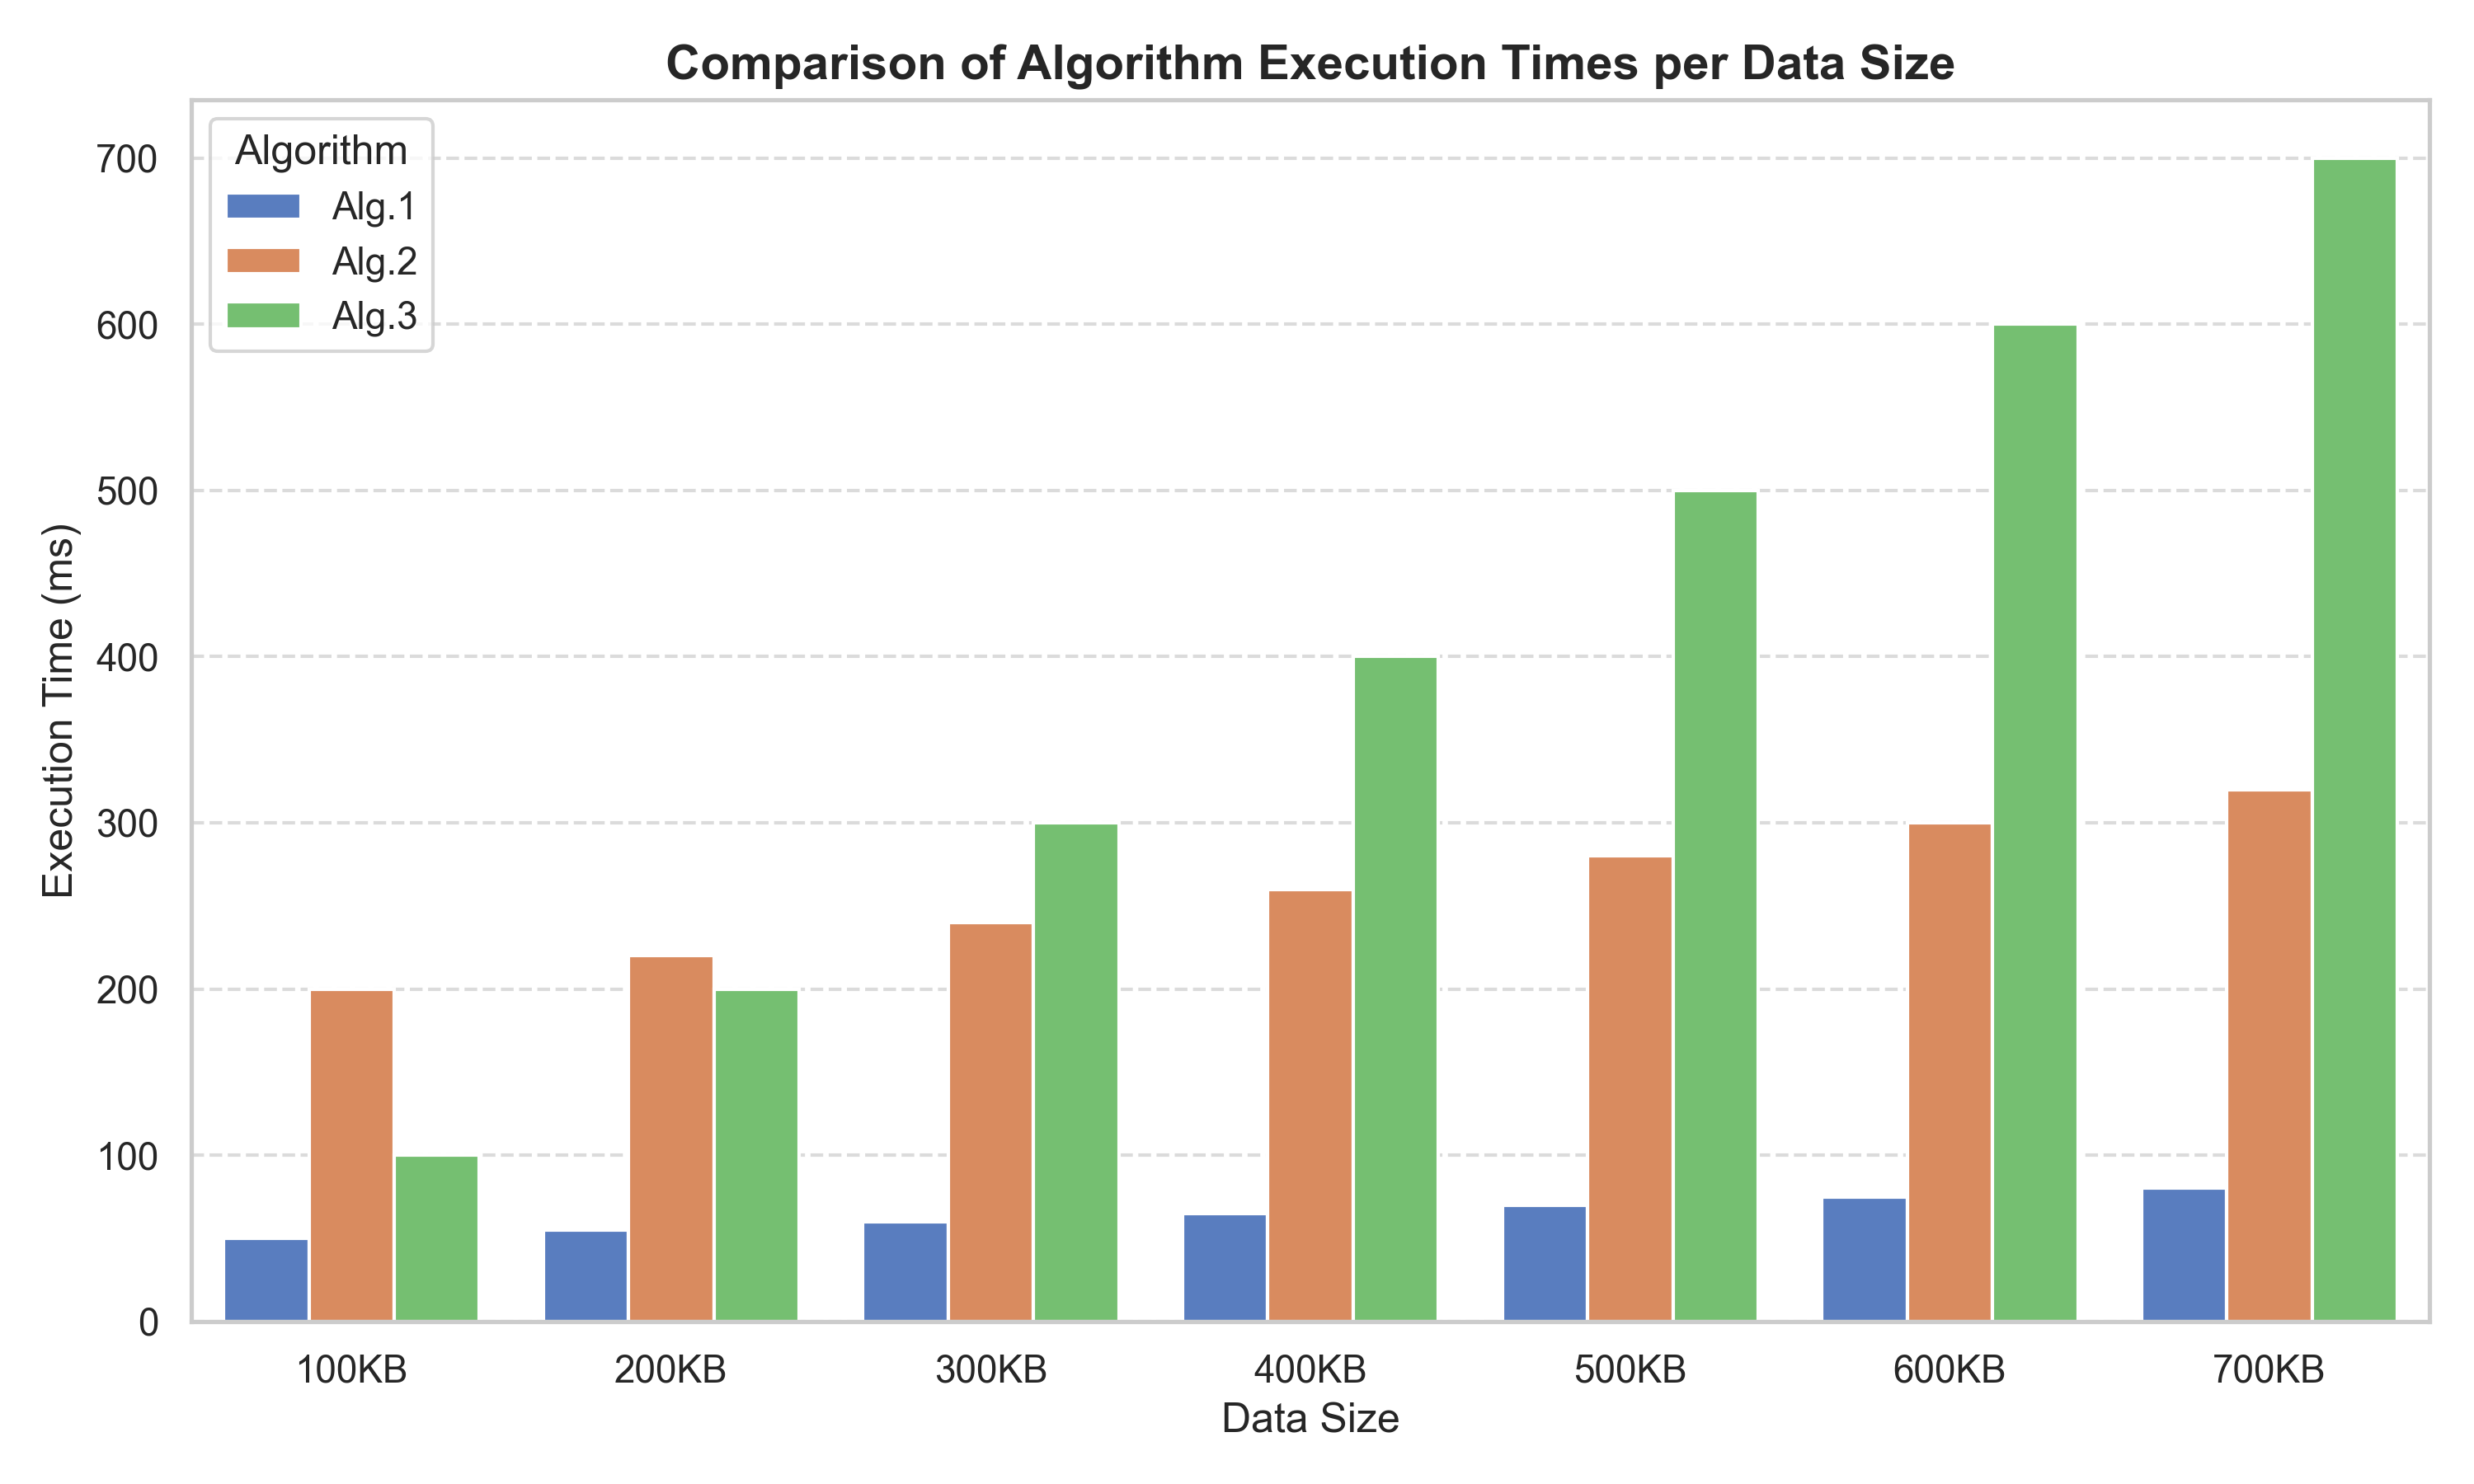
\includegraphics[width=0.85\textwidth]{execution_time_bar_plot.png}
    \caption{مقایسه ستونی و چندگانه زمان اجرای الگوریتم‌ها در هر یک از سطوح اندازه داده.}
    \label{fig:bar_plot}
\end{figure}

\begin{figure}[htbp]
    \centering
    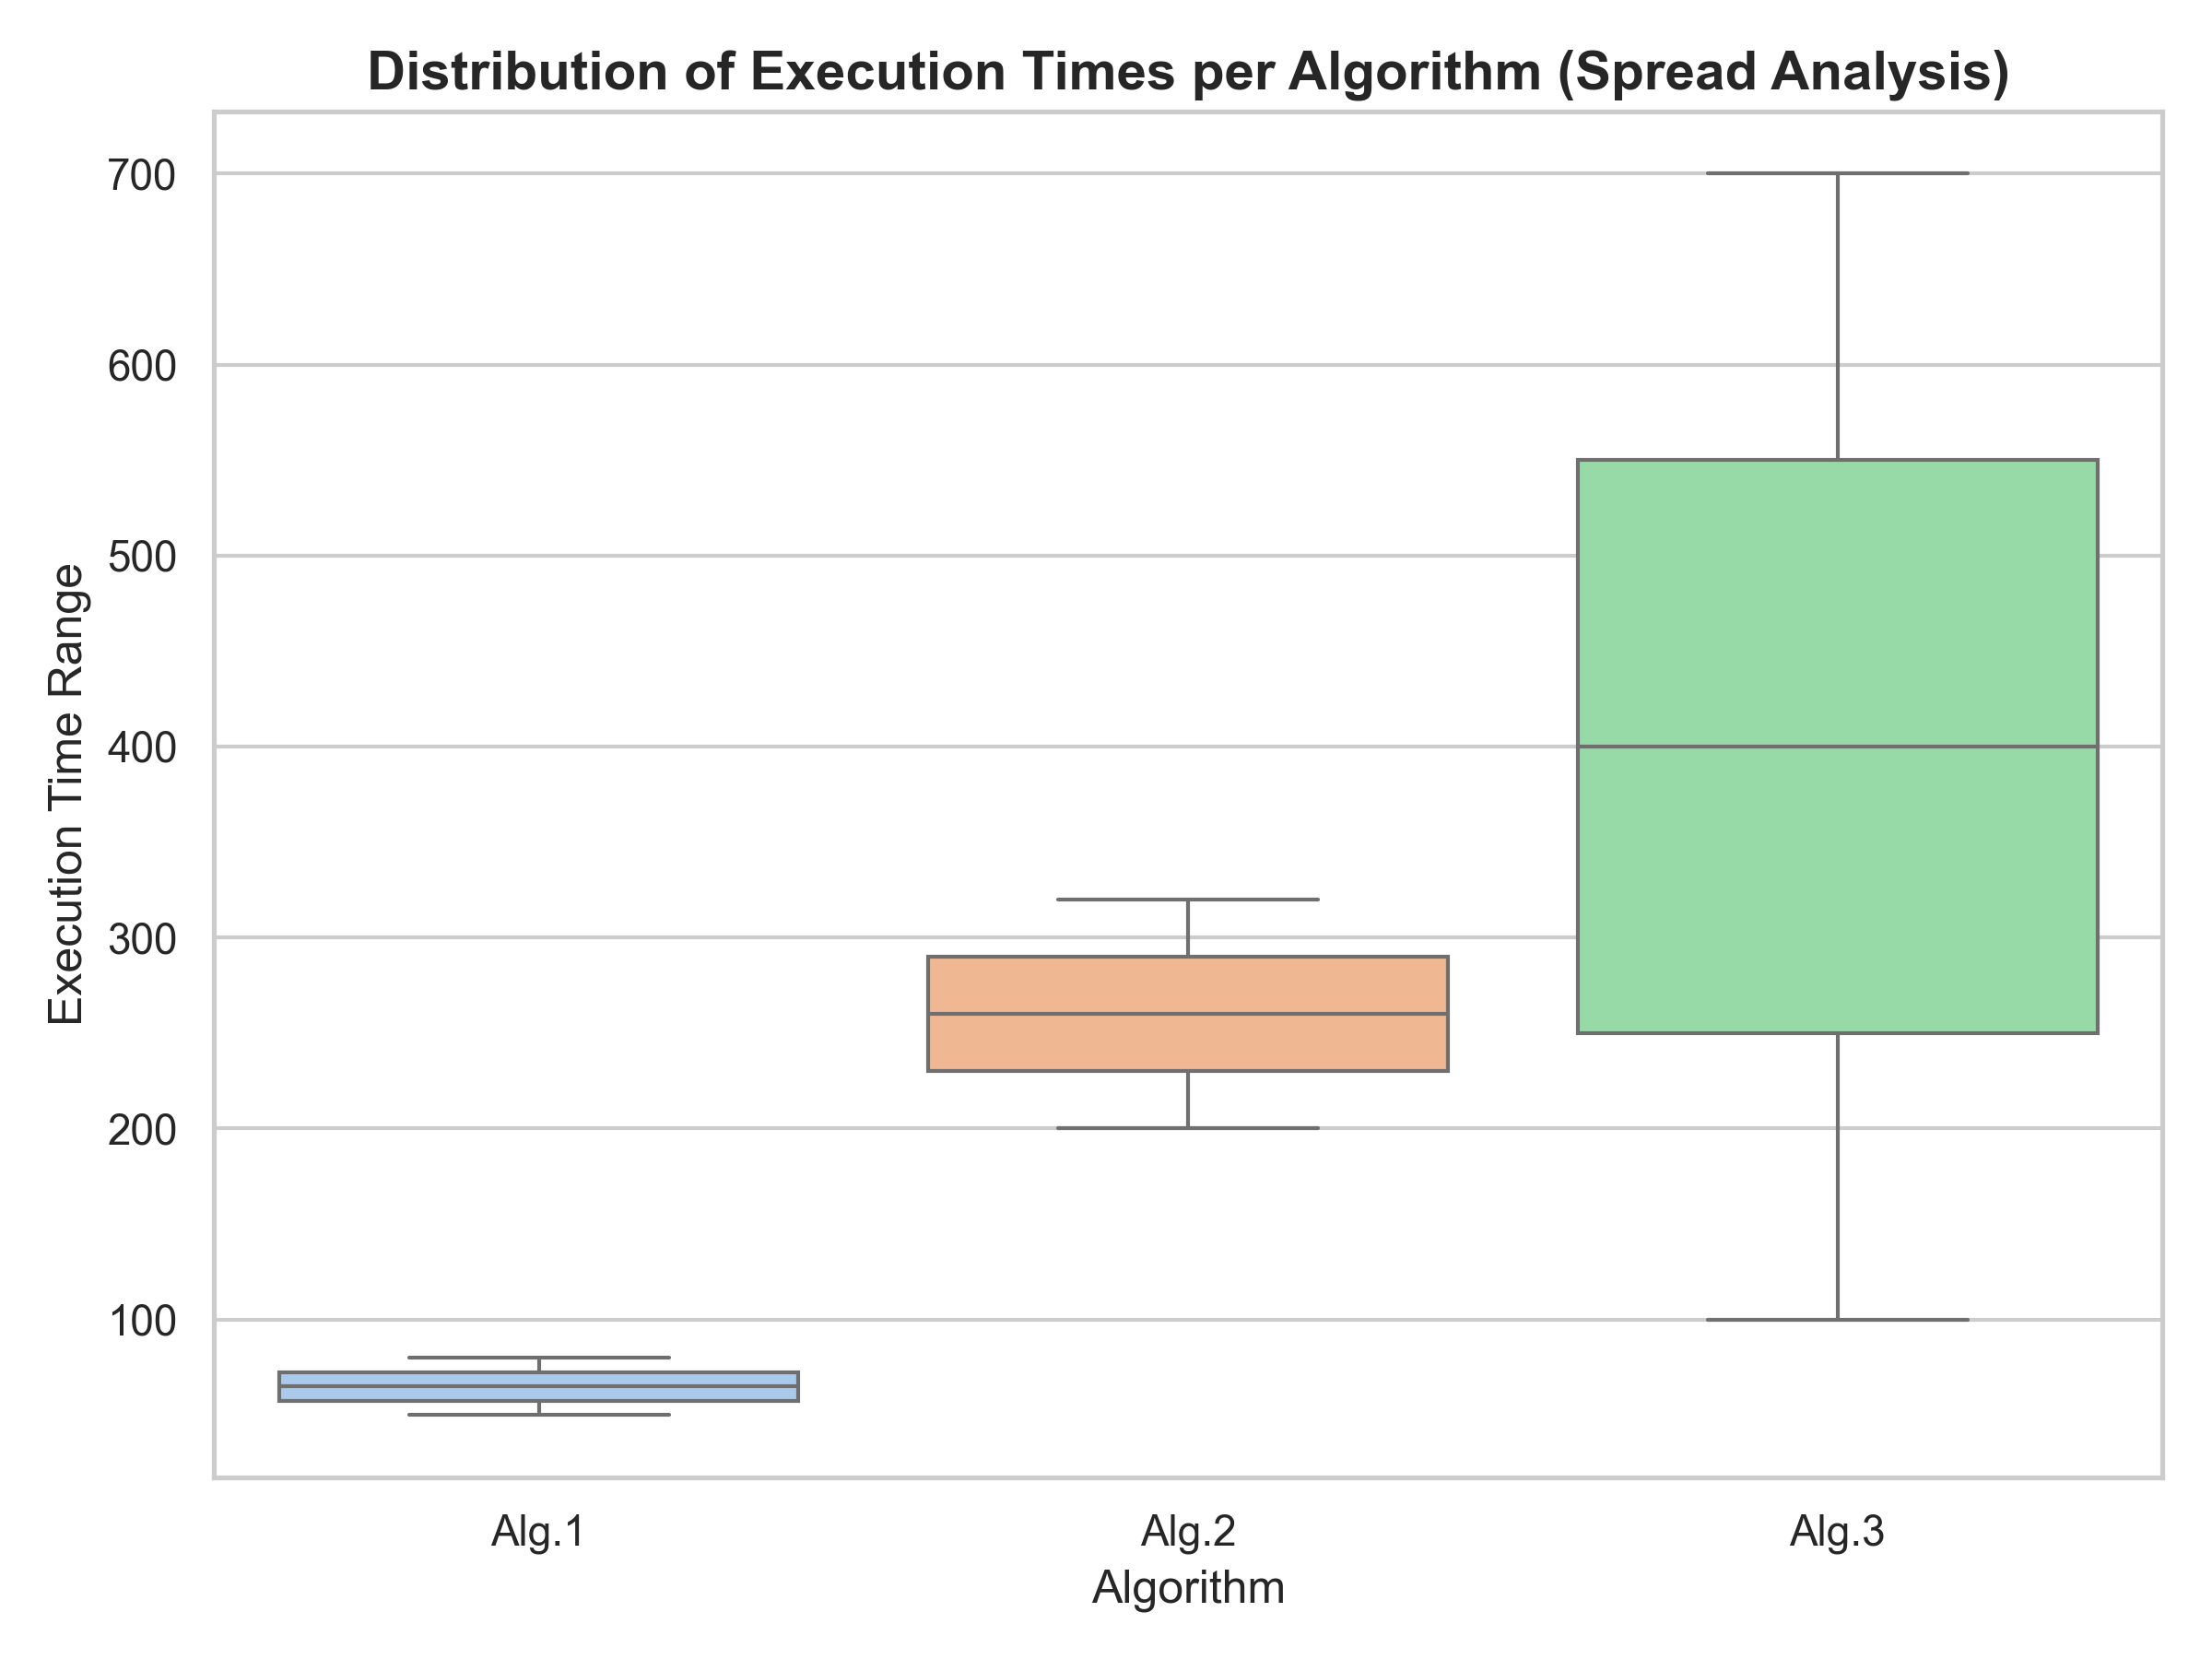
\includegraphics[width=0.7\textwidth]{execution_time_box_plot.png}
    \caption{نمودار جعبه‌ای تحلیل دامنه توزیع، میانه و پراکندگی کلی زمان اجرای الگوریتم‌ها.}
    \label{fig:box_plot}
\end{figure}

\subsubsection{تحلیل نمودار خطی و بررسی روند رشد}
با توجه به شکل~\ref{fig:line_plot}، رفتار رشد زمان اجرای هر سه الگوریتم به وضوح قابل تحلیل است:
\begin{itemize}
    \item \textbf{الگوریتم ۱:} این الگوریتم با شیبی بسیار ملایم رشد می‌کند و در تمام طول آزمایش کمترین زمان اجرا را به خود اختصاص داده است؛ در نتیجه، بهینه‌ترین الگوریتم از نظر پیچیدگی زمانی\footnote{\lr{Time Complexity}} است.
    \item \textbf{الگوریتم ۲:} روندی کاملاً خطی و با شیب ثابت دارد. اگرچه زمان شروع آن از الگوریتم ۳ در حجم‌های کوچک بیشتر است، اما نرخ رشد کنترل‌شده‌ای دارد.
    \item \textbf{الگوریتم ۳:} این الگوریتم دارای تندترین شیب صعودی است. زمان اجرای آن با افزایش اندازه ورودی به شدت بالا می‌رود و حالت ناپایداری در حجم‌های بزرگ پیدا می‌کند.
\end{itemize}

\subsubsection{تحلیل نمودار میله‌ای و مقایسه نقطه‌ای عملکرد}
بر اساس شکل~\ref{fig:bar_plot}، در اندازه‌های ورودی کوچک مانند $ 100 $ و $ 200 $ کیلوبایت، الگوریتم ۳ سریع‌تر از الگوریتم ۲ عمل می‌کند. اما یک نقطه تلاقی مهم در محدوده $ 300 $ کیلوبایت رخ می‌دهد. از حجم $ 400 $ کیلوبایت به بعد، الگوریتم ۲ گوی سبقت را از الگوریتم ۳ می‌رباید؛ چرا که زمان اجرای الگوریتم ۳ به شکل تصاعدی افزایش یافته و در حجم $ 700 $ کیلوبایت به اوج خود یعنی $ 700 $ میلی‌ثانیه می‌رسد. این امر عدم مقایس‌پذیری\footnote{\lr{Scalability}} الگوریتم ۳ را اثبات می‌کند.

\subsubsection{تحلیل نمودار جعبه‌ای و بررسی ثبات توزیع}
نمودار جعبه‌ای در شکل~\ref{fig:box_plot}، دامنه تغییرات داده‌ها را به تصویر می‌کشد:
\begin{itemize}
    \item جعبه مربوط به الگوریتم ۱\footnote{\lr{Alg.1}} بسیار فشرده و در پایین‌ترین سطح قرار دارد که نشان‌دهنده پایداری بالا، انحراف معیار ناچیز و واریانس بسیار کم در شرایط کاری مختلف است.
    \item جعبه مربوط به الگوریتم ۳\footnote{\lr{Alg.3}} بیشترین ارتفاع (طول بازه مابین چارک اول و سوم) را دارد. این گستردگی نشان‌دهنده حساسیت فوق‌العاده بالا و عدم ثبات زمان اجرای این الگوریتم نسبت به تغییر ابعاد ورودی سیستم است.
\end{itemize}

\clearpage
\section{انتگرال‌گیری عددی به روش‌های ذوزنقه‌ای، سیمپسون و کوادراتور گوسی}
در این بخش، هدف محاسبه عددی مقدار انتگرال تابع مشخص‌شده در صورت پروژه یعنی $ f(x) = e^{x^2} $ در بازه کران‌دار $ (0,1) $ است. از آنجا که این تابع فاقد پادمشتق برحسب توابع مقدماتی است، مقدار انتگرال آن صرفاً از طریق روش‌های تقریبی عددی محاسبه می‌شود. سه روش ذوزنقه‌ای\footnote{\lr{Trapezoidal Rule}}، سیمپسون\footnote{\lr{Simpson's Rule}} و کوادراتور گوسی\footnote{\lr{Gaussian Quadrature}} در محیط پایتون\footnote{\lr{Python}} روی این تابع اعمال شده‌اند.

\subsection{مراحل و نحوه پیاده‌سازی الگوریتم‌ها}
مراحل محاسباتی و الگوریتمی این بخش به شرح زیر است:
\begin{enumerate}
    \item \textbf{تعریف تابع هدف:} ابتدا تابع ریاضی $ f(x) = e^{x^2} $ با بهره‌گیری از تابع نمایی آرایه نام‌پای\footnote{\lr{NumPy}} یعنی \lstinline|np.exp| پیاده‌سازی می‌شود.
    \item \textbf{شبکه‌بندی بازه انتگرال‌گیری:} برای اعمال روش‌های مبتنی بر نیوتن-کوتس\footnote{\lr{Newton-Cotes formulas}} (ذوزنقه‌ای و سیمپسون)، بازه کل $ [0, 1] $ به کمک تابع \lstinline|np.linspace| به تعداد $ 100 $ زیربازه هم‌اندازه با مجموع $ 101 $ نقطه گره‌ای تقسیم‌بندی می‌شود.
    \item \textbf{اعمال قاعده‌ ذوزنقه‌ای و سیمپسون:} با استفاده از توابع اختصاصی و بهینه \lstinline|trapezoid| و \lstinline|simpson| از زیربسته محاسبات انتگرال سای‌پای\footnote{\lr{SciPy}} (\lstinline|scipy.integrate|)، ارزیابی عددی با دریافت فواصل نقشه گره‌ای انجام می‌پذیرد.
    \item \textbf{اعمال قاعده‌ کوادراتور گوس-کرونرود:} برای محاسبه انتگرال گوسی با بالاترین درجه دقت چندجمله‌ای، از تابع قدرتمند \lstinline|quad| استفاده شده است که علاوه بر مقدار انتگرال، تخمین دقیقی از خطای مطلق سقف محاسبات را نیز در خروجی برمی‌گرداند.
\end{enumerate}

\subsection{کد پایتون پیاده‌سازی شده}
کد کامل پایتون توسعه‌یافته برای محاسبات انتگرال‌گیری عددی به شرح زیر است:

\begin{latin}
\begin{lstlisting}
import numpy as np
from scipy.integrate import trapezoid, simpson, quad

# 1. Define the target function f(x) = e^(x^2)
def f(x):
    return np.exp(x**2)

# Define the integration intervals (from 0 to 1)
a = 0
b = 1

# Number of points for Trapezoidal and Simpson's methods
num_points = 101
x_intervals = np.linspace(a, b, num_points)
y_values = f(x_intervals)

print("--- Part 3 (a): Trapezoidal and Simpson's Methods ---")

# 2. Calculate using the Trapezoidal Rule
integral_trapezoidal = trapezoid(y_values, x_intervals)
print(f"Trapezoidal Rule Result: {integral_trapezoidal:.8f}")

# 3. Calculate using Simpson's Rule
integral_simpson = simpson(y_values, x_intervals)
print(f"Simpson's Rule Result:    {integral_simpson:.8f}\n")

print("--- Part 3 (b): Gaussian Quadrature Method ---")

# 4. Calculate using Gaussian Quadrature
integral_gaussian, abs_error = quad(f, a, b)
print(f"Gaussian Quadrature Result: {integral_gaussian:.8f}")
print(f"Estimated Absolute Error:    {abs_error:.2e}\n")

print("--- Summary & Comparison ---")
print(f"Difference (Gaussian vs Simpson):     {abs(integral_gaussian - integral_simpson):.2e}")
print(f"Difference (Gaussian vs Trapezoidal): {abs(integral_gaussian - integral_trapezoidal):.2e}")
\end{lstlisting}
\end{latin}

\subsection{خروجی دقیق برنامه در محیط ترمینال}
مقادیر عددی خروجی چاپ‌شده در ترمینال پس از اجرای اسکریپت فوق به صورت زیر ثبت شده است:

\begin{latin}
\begin{verbatim}
--- Part 3 (a): Trapezoidal and Simpson's Methods ---
Trapezoidal Rule Result: 1.46269705
Simpson's Rule Result:    1.46265175

--- Part 3 (b): Gaussian Quadrature Method ---
Gaussian Quadrature Result: 1.46265175
Estimated Absolute Error:    1.62e-14

--- Summary & Comparison ---
Difference (Gaussian vs Simpson):     3.02e-09
Difference (Gaussian vs Trapezoidal): 4.53e-05
\end{verbatim}
\end{latin}

\subsection{تحلیل و مقایسه جامع نتایج عددی روش‌ها}
با توجه به نتایج حاصل از خروجی سیستم، مقدار تقریبی انتگرال برای هر سه روش با دقت اعشاری بالا استخراج گردید. فرمول ریاضی هر یک از روش‌ها و تحلیل خطای آن‌ها به شرح زیر تبیین می‌شود.

\subsubsection{روش ذوزنقه‌ای}
در این روش، تابع در هر زیربازه با یک خط راست تقریب زده می‌شود. فرمول محاسباتی آن به صورت زیر است:
\[
I_T = \frac{h}{2} \left[ f(x_0) + 2\sum_{i=1}^{n-1} f(x_i) + f(x_n) \right].
\]
مقدار حاصل از این روش برابر با $ 1.46269705 $ به‌دست آمده است. این روش به دلیل استفاده از تقریب‌های مرتبه اول خطی، دارای خطای قطع کلی از مرتبه $ \mathcal{O}(h^2) $ است. تفاوت این روش با روش گوسی برابر با $ 4.53 \times 10^{-5} $ است که بیشترین میزان انحراف را در میان روش‌های مورد آزمایش نشان می‌دهد.

\subsubsection{روش سیمپسون}
در روش سیمپسون، تقریب توابع در هر دو زیربازه مجاور با استفاده از سهمی‌های درجه دوم انجام می‌گیرد. فرمول ریاضی این قاعده به صورت زیر است:
\[
I_S = \frac{h}{3} \left[ f(x_0) + 4\sum_{i=1,3,\dots}^{n-1} f(x_i) + 2\sum_{j=2,4,\dots}^{n-2} f(x_j) + f(x_n) \right].
\]
مقدار عددی حاصل از محاسبات سیمپسون برابر با $ 1.46265175 $ است. خطای قطع این روش از مرتبه $ \mathcal{O}(h^4) $ است. به دلیل انحنای سهموی توابع برازش شده، این روش انطباق بسیار بالایی با ساختار هموار تابع $ e^{x^2} $ دارد، به طوری که تفاوت خروجی آن با روش گوسی صرفاً برابر با $ 3.02 \times 10^{-9} $ است که نشان‌دهنده دقت فوق‌العاده بالای آن در تعداد بازه داده‌شده است.

\subsubsection{روش کوادراتور گوسی}
روش کوادراتور گوسی برخلاف دو روش قبل که از فواصل یکنواخت و ثابت استفاده می‌کردند، نقاط نمونه‌برداری $ x_i $ و وزن‌های متناظر $ w_i $ را به صورت بهینه و بر اساس ریشه‌های چندجمله‌ای‌های لژاندر\footnote{\lr{Legendre polynomials}} انتخاب می‌کند تا چندجمله‌ای‌های درجه بالا را دقیقاً انتگرال‌گیری کند:
\[
I_G = \sum_{i=1}^{m} w_i f(x_i).
\]
مقدار حاصل از این روش دقیق برابر با $ 1.46265175 $ با مرتبه خطای فوق‌العاده ناچیز و حد آستانه خطای مطلق محاسباتی معادل $ 1.62 \times 10^{-14} $ به‌دست آمده است. 

\subsubsection{نتیجه‌گیری مقایسه‌ای}
با در نظر گرفتن روش کوادراتور گوسی به عنوان دقیق‌ترین معیار انتگرال‌گیری عددی (به دلیل ساختار متغیر و بهینه نقاط ارزیابی)، مقایسه شاخص‌ها اثبات می‌کند که روش سیمپسون با داشتن خطای ناچیز مرتبه نهم، به طرز چشمگیری نسبت به روش ذوزنقه‌ای (با خطای مرتبه پنجم) ارجحیت دارد. دلیل این امر، نرم بودن و مشتق‌پذیری بی‌نهایت تابع تحت انتگرال است که باعث می‌شود فرمول‌های مرتبه بالاتر مانند سیمپسون و کوادراتور گوسی با سرعت بسیار بالاتری به سمت مقدار واقعی انتگرال همگرا شوند.


\end{document}
